\documentclass{standalone}
\usepackage{tikz}
\usetikzlibrary{patterns}
\usetikzlibrary{positioning}
\usetikzlibrary{patterns, positioning}
\usetikzlibrary{shapes.misc}
\usepackage[outline]{contour}
\contourlength{1.5pt} 
\usetikzlibrary{calc}
        \usepackage{relsize}
        \tikzset{fontscale/.style = {font=\relsize{#1}}}

\begin{document}
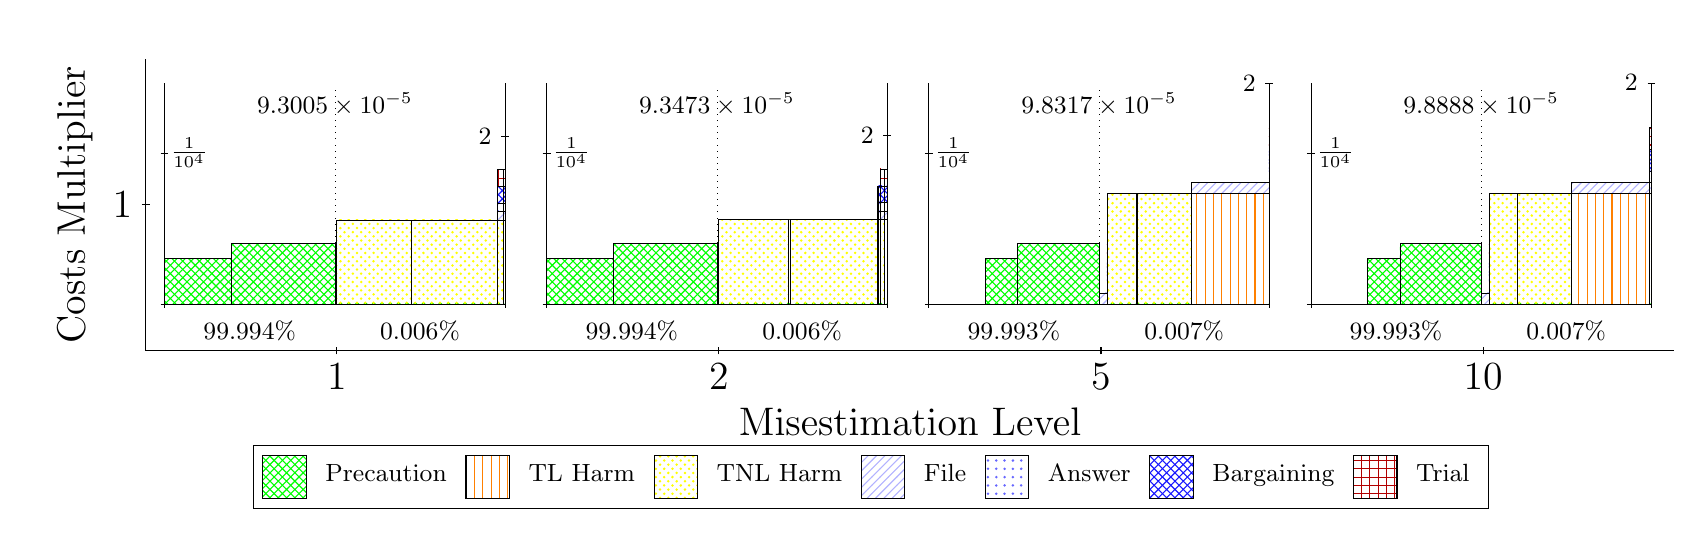
\begin{tikzpicture}
\clip(-0.5,-1.1) rectangle +(20.91,6.2);
\draw[black] (1,1) -- (1,4.7);
\node[rotate=90, fontscale=2, anchor=center] at (0.1, 2.85) {Costs Multiplier};
\draw[black] (0.95,2.85) -- (1.05,2.85);
\node[fontscale=2, anchor=east] at (0.95, 2.85) {1};

\draw[black] (1,1) -- (20.41,1);
\node[fontscale=2, anchor=center] at (10.705, 0.1) {Misestimation Level};
\draw[black] (3.4263,0.95) -- (3.4263,1.05);
\node[fontscale=2, anchor=north] at (3.4263, 0.95) {1};
\draw[black] (8.2788,0.95) -- (8.2788,1.05);
\node[fontscale=2, anchor=north] at (8.2788, 0.95) {2};
\draw[black] (13.131,0.95) -- (13.131,1.05);
\node[fontscale=2, anchor=north] at (13.131, 0.95) {5};
\draw[black] (17.984,0.95) -- (17.984,1.05);
\node[fontscale=2, anchor=north] at (17.984, 0.95) {10};


\draw[pattern=crosshatch, pattern color=green,draw=black,very thin] (1.2381,1.592) rectangle (2.0858,2.1671);
\draw[pattern=crosshatch, pattern color=green,draw=black,very thin] (2.0858,1.592) rectangle (3.4013,2.3588);
\draw[pattern=crosshatch, pattern color=green,draw=black,very thin] (3.4013,1.592) rectangle (3.4172,1.592);
\draw[pattern=north east lines, pattern color=blue!30,draw=black,very thin] (3.4013,1.592) rectangle (3.4172,1.6986);
\draw[pattern=dots,  pattern color=blue!60,draw=black,very thin] (3.4013,1.6986) rectangle (3.4172,1.8052);
\draw[pattern=crosshatch,      pattern color=blue!90,draw=black,very thin] (3.4013,1.8052) rectangle (3.4172,2.0184);
\draw[pattern=grid,            pattern color=red!70!black,draw=black,very thin] (3.4013,2.0184) rectangle (3.4172,2.2316);
\draw[pattern=crosshatch, pattern color=green,draw=black,very thin] (3.4172,1.592) rectangle (4.3666,1.592);
\draw[pattern=crosshatch dots, pattern color=yellow,draw=black,very thin] (3.4172,1.592) rectangle (4.3666,2.658);
\draw[pattern=crosshatch, pattern color=green,draw=black,very thin] (4.3666,1.592) rectangle (4.3766,1.592);
\draw[pattern=vertical lines, pattern color=orange,draw=black,very thin] (4.3666,1.592) rectangle (4.3766,2.658);
\draw[pattern=crosshatch, pattern color=green,draw=black,very thin] (4.3766,1.592) rectangle (5.4682,1.592);
\draw[pattern=crosshatch dots, pattern color=yellow,draw=black,very thin] (4.3766,1.592) rectangle (5.4682,2.658);
\draw[pattern=crosshatch, pattern color=green,draw=black,very thin] (5.4682,1.592) rectangle (5.5394,1.592);
\draw[pattern=crosshatch dots, pattern color=yellow,draw=black,very thin] (5.4682,1.592) rectangle (5.5394,2.658);
\draw[pattern=north east lines, pattern color=blue!30,draw=black,very thin] (5.4682,2.658) rectangle (5.5394,2.7646);
\draw[pattern=dots,  pattern color=blue!60,draw=black,very thin] (5.4682,2.7646) rectangle (5.5394,2.8712);
\draw[pattern=crosshatch,      pattern color=blue!90,draw=black,very thin] (5.4682,2.8712) rectangle (5.5394,3.0844);
\draw[pattern=grid,            pattern color=red!70!black,draw=black,very thin] (5.4682,3.0844) rectangle (5.5394,3.2976);
\draw[pattern=crosshatch, pattern color=green,draw=black,very thin] (5.5394,1.592) rectangle (5.5644,1.592);
\draw[pattern=vertical lines, pattern color=orange,draw=black,very thin] (5.5394,1.592) rectangle (5.5644,2.658);
\draw[pattern=north east lines, pattern color=blue!30,draw=black,very thin] (5.5394,2.658) rectangle (5.5644,2.7646);
\draw[pattern=dots,  pattern color=blue!60,draw=black,very thin] (5.5394,2.7646) rectangle (5.5644,2.8712);
\draw[pattern=crosshatch,      pattern color=blue!90,draw=black,very thin] (5.5394,2.8712) rectangle (5.5644,3.0844);
\draw[pattern=grid,            pattern color=red!70!black,draw=black,very thin] (5.5394,3.0844) rectangle (5.5644,3.2976);
\node[font=\small,text=black,anchor=north] at (3.4013, 4.4) {$9.3005\times 10^{-5}$};
\draw[black,very thin] (1.2381,1.592) -- (1.2381,4.4);
\draw[black,very thin] (1.1881,1.592) -- (1.2881,1.592);
\node[font=\small,text=black, anchor=west] at (1.1881, 1.592) {};
\draw[black,very thin] (1.1881,3.509) -- (1.2881,3.509);
\node[font=\small,text=black, anchor=west] at (1.1881, 3.509) {$\frac{1}{10^{4}}$};

\draw[black,dotted,very thin] (3.4013,1.6762) -- (3.4013,4.3158);
\draw[black,very thin] (5.5644,1.592) -- (5.5644,4.4);
\draw[black,very thin] (5.5144,3.724) -- (5.6144,3.724);
\node[font=\small,text=black, anchor=east] at (5.5144, 3.724) {\contour{white}{2}};

\draw[black,very thin] (1.2381,1.592) -- (5.5644,1.592);
\draw[black,very thin] (1.2381,1.542) -- (1.2381,1.642);
\node[font=\small,text=black, anchor=north] at (1.2381, 1.542) {};
\draw[black,very thin] (5.5644,1.542) -- (5.5644,1.642);
\node[font=\small,text=black, anchor=north] at (5.5644, 1.542) {};

\node[font=\small,text=black,anchor=south] at (2.3197, 0.992) {99.994\%};
\node[font=\small,text=black,anchor=south] at (4.4828, 0.992) {0.006\%};

\draw[pattern=crosshatch, pattern color=green,draw=black,very thin] (6.0906,1.592) rectangle (6.9387,2.1671);
\draw[pattern=crosshatch, pattern color=green,draw=black,very thin] (6.9387,1.592) rectangle (8.2538,2.3588);
\draw[pattern=crosshatch, pattern color=green,draw=black,very thin] (8.2538,1.592) rectangle (8.2602,1.592);
\draw[pattern=north east lines, pattern color=blue!30,draw=black,very thin] (8.2538,1.592) rectangle (8.2602,1.6992);
\draw[pattern=dots,  pattern color=blue!60,draw=black,very thin] (8.2538,1.6992) rectangle (8.2602,1.8063);
\draw[pattern=crosshatch,      pattern color=blue!90,draw=black,very thin] (8.2538,1.8063) rectangle (8.2602,2.0205);
\draw[pattern=crosshatch, pattern color=green,draw=black,very thin] (8.2602,1.592) rectangle (8.2756,1.592);
\draw[pattern=north east lines, pattern color=blue!30,draw=black,very thin] (8.2602,1.592) rectangle (8.2756,1.6992);
\draw[pattern=dots,  pattern color=blue!60,draw=black,very thin] (8.2602,1.6992) rectangle (8.2756,1.8063);
\draw[pattern=crosshatch,      pattern color=blue!90,draw=black,very thin] (8.2602,1.8063) rectangle (8.2756,2.0205);
\draw[pattern=grid,            pattern color=red!70!black,draw=black,very thin] (8.2602,2.0205) rectangle (8.2756,2.2348);
\draw[pattern=crosshatch, pattern color=green,draw=black,very thin] (8.2756,1.592) rectangle (9.1597,1.592);
\draw[pattern=crosshatch dots, pattern color=yellow,draw=black,very thin] (8.2756,1.592) rectangle (9.1597,2.6633);
\draw[pattern=crosshatch, pattern color=green,draw=black,very thin] (9.1597,1.592) rectangle (9.1805,1.592);
\draw[pattern=vertical lines, pattern color=orange,draw=black,very thin] (9.1597,1.592) rectangle (9.1805,2.6633);
\draw[pattern=crosshatch, pattern color=green,draw=black,very thin] (9.1805,1.592) rectangle (10.29,1.592);
\draw[pattern=crosshatch dots, pattern color=yellow,draw=black,very thin] (9.1805,1.592) rectangle (10.29,2.6633);
\draw[pattern=crosshatch, pattern color=green,draw=black,very thin] (10.29,1.592) rectangle (10.306,1.592);
\draw[pattern=crosshatch dots, pattern color=yellow,draw=black,very thin] (10.29,1.592) rectangle (10.306,2.6633);
\draw[pattern=north east lines, pattern color=blue!30,draw=black,very thin] (10.29,2.6633) rectangle (10.306,2.7704);
\draw[pattern=dots,  pattern color=blue!60,draw=black,very thin] (10.29,2.7704) rectangle (10.306,2.8775);
\draw[pattern=crosshatch,      pattern color=blue!90,draw=black,very thin] (10.29,2.8775) rectangle (10.306,3.0917);
\draw[pattern=crosshatch, pattern color=green,draw=black,very thin] (10.306,1.592) rectangle (10.326,1.592);
\draw[pattern=vertical lines, pattern color=orange,draw=black,very thin] (10.306,1.592) rectangle (10.326,2.6633);
\draw[pattern=north east lines, pattern color=blue!30,draw=black,very thin] (10.306,2.6633) rectangle (10.326,2.7704);
\draw[pattern=dots,  pattern color=blue!60,draw=black,very thin] (10.306,2.7704) rectangle (10.326,2.8775);
\draw[pattern=crosshatch,      pattern color=blue!90,draw=black,very thin] (10.306,2.8775) rectangle (10.326,3.0917);
\draw[pattern=crosshatch, pattern color=green,draw=black,very thin] (10.326,1.592) rectangle (10.384,1.592);
\draw[pattern=crosshatch dots, pattern color=yellow,draw=black,very thin] (10.326,1.592) rectangle (10.384,2.6633);
\draw[pattern=north east lines, pattern color=blue!30,draw=black,very thin] (10.326,2.6633) rectangle (10.384,2.7704);
\draw[pattern=dots,  pattern color=blue!60,draw=black,very thin] (10.326,2.7704) rectangle (10.384,2.8775);
\draw[pattern=crosshatch,      pattern color=blue!90,draw=black,very thin] (10.326,2.8775) rectangle (10.384,3.0917);
\draw[pattern=grid,            pattern color=red!70!black,draw=black,very thin] (10.326,3.0917) rectangle (10.384,3.306);
\draw[pattern=crosshatch, pattern color=green,draw=black,very thin] (10.384,1.592) rectangle (10.417,1.592);
\draw[pattern=vertical lines, pattern color=orange,draw=black,very thin] (10.384,1.592) rectangle (10.417,2.6633);
\draw[pattern=north east lines, pattern color=blue!30,draw=black,very thin] (10.384,2.6633) rectangle (10.417,2.7704);
\draw[pattern=dots,  pattern color=blue!60,draw=black,very thin] (10.384,2.7704) rectangle (10.417,2.8775);
\draw[pattern=crosshatch,      pattern color=blue!90,draw=black,very thin] (10.384,2.8775) rectangle (10.417,3.0917);
\draw[pattern=grid,            pattern color=red!70!black,draw=black,very thin] (10.384,3.0917) rectangle (10.417,3.306);
\node[font=\small,text=black,anchor=north] at (8.2538, 4.4) {$9.3473\times 10^{-5}$};
\draw[black,very thin] (6.0906,1.592) -- (6.0906,4.4);
\draw[black,very thin] (6.0406,1.592) -- (6.1406,1.592);
\node[font=\small,text=black, anchor=west] at (6.0406, 1.592) {};
\draw[black,very thin] (6.0406,3.509) -- (6.1406,3.509);
\node[font=\small,text=black, anchor=west] at (6.0406, 3.509) {$\frac{1}{10^{4}}$};

\draw[black,dotted,very thin] (8.2538,1.6762) -- (8.2538,4.3158);
\draw[black,very thin] (10.417,1.592) -- (10.417,4.4);
\draw[black,very thin] (10.367,3.7344) -- (10.467,3.7344);
\node[font=\small,text=black, anchor=east] at (10.367, 3.7344) {\contour{white}{2}};

\draw[black,very thin] (6.0906,1.592) -- (10.417,1.592);
\draw[black,very thin] (6.0906,1.542) -- (6.0906,1.642);
\node[font=\small,text=black, anchor=north] at (6.0906, 1.542) {};
\draw[black,very thin] (10.417,1.542) -- (10.417,1.642);
\node[font=\small,text=black, anchor=north] at (10.417, 1.542) {};

\node[font=\small,text=black,anchor=south] at (7.1722, 0.992) {99.994\%};
\node[font=\small,text=black,anchor=south] at (9.3353, 0.992) {0.006\%};

\draw[pattern=crosshatch, pattern color=green,draw=black,very thin] (11.664,1.592) rectangle (12.074,2.1671);
\draw[pattern=crosshatch, pattern color=green,draw=black,very thin] (12.074,1.592) rectangle (13.106,2.3588);
\draw[pattern=north east lines, pattern color=blue!30,draw=black,very thin] (13.106,1.592) rectangle (13.205,1.7321);
\draw[pattern=crosshatch, pattern color=green,draw=black,very thin] (13.205,1.592) rectangle (13.206,1.592);
\draw[pattern=north east lines, pattern color=blue!30,draw=black,very thin] (13.205,1.592) rectangle (13.206,1.7322);
\draw[pattern=dots,  pattern color=blue!60,draw=black,very thin] (13.205,1.7322) rectangle (13.206,1.8723);
\draw[pattern=crosshatch,      pattern color=blue!90,draw=black,very thin] (13.205,1.8723) rectangle (13.206,2.1526);
\draw[pattern=grid,            pattern color=red!70!black,draw=black,very thin] (13.205,2.1526) rectangle (13.206,2.4329);
\draw[pattern=crosshatch, pattern color=green,draw=black,very thin] (13.206,1.592) rectangle (13.585,1.592);
\draw[pattern=crosshatch dots, pattern color=yellow,draw=black,very thin] (13.206,1.592) rectangle (13.585,2.9935);
\draw[pattern=crosshatch, pattern color=green,draw=black,very thin] (13.585,1.592) rectangle (13.592,1.592);
\draw[pattern=vertical lines, pattern color=orange,draw=black,very thin] (13.585,1.592) rectangle (13.592,2.9935);
\draw[pattern=crosshatch, pattern color=green,draw=black,very thin] (13.592,1.592) rectangle (14.277,1.5921);
\draw[pattern=crosshatch dots, pattern color=yellow,draw=black,very thin] (13.592,1.5921) rectangle (14.277,2.9935);
\draw[pattern=vertical lines, pattern color=orange,draw=black,very thin] (14.277,1.592) rectangle (15.263,2.9934);
\draw[pattern=north east lines, pattern color=blue!30,draw=black,very thin] (14.277,2.9934) rectangle (15.263,3.1336);
\draw[pattern=crosshatch, pattern color=green,draw=black,very thin] (15.263,1.592) rectangle (15.267,1.592);
\draw[pattern=crosshatch dots, pattern color=yellow,draw=black,very thin] (15.263,1.592) rectangle (15.267,2.9935);
\draw[pattern=north east lines, pattern color=blue!30,draw=black,very thin] (15.263,2.9935) rectangle (15.267,3.1336);
\draw[pattern=dots,  pattern color=blue!60,draw=black,very thin] (15.263,3.1336) rectangle (15.267,3.2738);
\draw[pattern=crosshatch,      pattern color=blue!90,draw=black,very thin] (15.263,3.2738) rectangle (15.267,3.554);
\draw[pattern=grid,            pattern color=red!70!black,draw=black,very thin] (15.263,3.554) rectangle (15.267,3.8343);
\draw[pattern=crosshatch, pattern color=green,draw=black,very thin] (15.267,1.592) rectangle (15.269,1.592);
\draw[pattern=vertical lines, pattern color=orange,draw=black,very thin] (15.267,1.592) rectangle (15.269,2.9935);
\draw[pattern=north east lines, pattern color=blue!30,draw=black,very thin] (15.267,2.9935) rectangle (15.269,3.1336);
\draw[pattern=dots,  pattern color=blue!60,draw=black,very thin] (15.267,3.1336) rectangle (15.269,3.2738);
\draw[pattern=crosshatch,      pattern color=blue!90,draw=black,very thin] (15.267,3.2738) rectangle (15.269,3.554);
\draw[pattern=grid,            pattern color=red!70!black,draw=black,very thin] (15.267,3.554) rectangle (15.269,3.8343);
\node[font=\small,text=black,anchor=north] at (13.106, 4.4) {$9.8317\times 10^{-5}$};
\draw[black,very thin] (10.943,1.592) -- (10.943,4.4);
\draw[black,very thin] (10.893,1.592) -- (10.993,1.592);
\node[font=\small,text=black, anchor=west] at (10.893, 1.592) {};
\draw[black,very thin] (10.893,3.509) -- (10.993,3.509);
\node[font=\small,text=black, anchor=west] at (10.893, 3.509) {$\frac{1}{10^{4}}$};

\draw[black,dotted,very thin] (13.106,1.6762) -- (13.106,4.3158);
\draw[black,very thin] (15.269,1.592) -- (15.269,4.4);
\draw[black,very thin] (15.219,4.3948) -- (15.319,4.3948);
\node[font=\small,text=black, anchor=east] at (15.219, 4.3948) {\contour{white}{2}};

\draw[black,very thin] (10.943,1.592) -- (15.269,1.592);
\draw[black,very thin] (10.943,1.542) -- (10.943,1.642);
\node[font=\small,text=black, anchor=north] at (10.943, 1.542) {};
\draw[black,very thin] (15.269,1.542) -- (15.269,1.642);
\node[font=\small,text=black, anchor=north] at (15.269, 1.542) {};

\node[font=\small,text=black,anchor=south] at (12.025, 0.992) {99.993\%};
\node[font=\small,text=black,anchor=south] at (14.188, 0.992) {0.007\%};

\draw[pattern=crosshatch, pattern color=green,draw=black,very thin] (16.517,1.592) rectangle (16.926,2.1671);
\draw[pattern=crosshatch, pattern color=green,draw=black,very thin] (16.926,1.592) rectangle (17.959,2.3588);
\draw[pattern=north east lines, pattern color=blue!30,draw=black,very thin] (17.959,1.592) rectangle (18.057,1.7324);
\draw[pattern=crosshatch, pattern color=green,draw=black,very thin] (18.057,1.592) rectangle (18.062,1.592);
\draw[pattern=north east lines, pattern color=blue!30,draw=black,very thin] (18.057,1.592) rectangle (18.062,1.7324);
\draw[pattern=dots,  pattern color=blue!60,draw=black,very thin] (18.057,1.7324) rectangle (18.062,1.8728);
\draw[pattern=crosshatch,      pattern color=blue!90,draw=black,very thin] (18.057,1.8728) rectangle (18.062,2.1536);
\draw[pattern=grid,            pattern color=red!70!black,draw=black,very thin] (18.057,2.1536) rectangle (18.062,2.4344);
\draw[pattern=crosshatch, pattern color=green,draw=black,very thin] (18.062,1.592) rectangle (18.421,1.592);
\draw[pattern=crosshatch dots, pattern color=yellow,draw=black,very thin] (18.062,1.592) rectangle (18.421,2.996);
\draw[pattern=crosshatch, pattern color=green,draw=black,very thin] (18.421,1.592) rectangle (18.423,1.592);
\draw[pattern=vertical lines, pattern color=orange,draw=black,very thin] (18.421,1.592) rectangle (18.423,2.996);
\draw[pattern=crosshatch, pattern color=green,draw=black,very thin] (18.423,1.592) rectangle (19.107,1.5921);
\draw[pattern=crosshatch dots, pattern color=yellow,draw=black,very thin] (18.423,1.5921) rectangle (19.107,2.996);
\draw[pattern=vertical lines, pattern color=orange,draw=black,very thin] (19.107,1.592) rectangle (20.092,2.996);
\draw[pattern=north east lines, pattern color=blue!30,draw=black,very thin] (19.107,2.996) rectangle (20.092,3.1364);
\draw[pattern=crosshatch, pattern color=green,draw=black,very thin] (20.092,1.592) rectangle (20.115,1.592);
\draw[pattern=crosshatch dots, pattern color=yellow,draw=black,very thin] (20.092,1.592) rectangle (20.115,2.996);
\draw[pattern=north east lines, pattern color=blue!30,draw=black,very thin] (20.092,2.996) rectangle (20.115,3.1364);
\draw[pattern=dots,  pattern color=blue!60,draw=black,very thin] (20.092,3.1364) rectangle (20.115,3.2768);
\draw[pattern=crosshatch,      pattern color=blue!90,draw=black,very thin] (20.092,3.2768) rectangle (20.115,3.5576);
\draw[pattern=grid,            pattern color=red!70!black,draw=black,very thin] (20.092,3.5576) rectangle (20.115,3.8384);
\draw[pattern=crosshatch, pattern color=green,draw=black,very thin] (20.115,1.592) rectangle (20.122,1.592);
\draw[pattern=vertical lines, pattern color=orange,draw=black,very thin] (20.115,1.592) rectangle (20.122,2.996);
\draw[pattern=north east lines, pattern color=blue!30,draw=black,very thin] (20.115,2.996) rectangle (20.122,3.1364);
\draw[pattern=dots,  pattern color=blue!60,draw=black,very thin] (20.115,3.1364) rectangle (20.122,3.2768);
\draw[pattern=crosshatch,      pattern color=blue!90,draw=black,very thin] (20.115,3.2768) rectangle (20.122,3.5576);
\draw[pattern=grid,            pattern color=red!70!black,draw=black,very thin] (20.115,3.5576) rectangle (20.122,3.8384);
\node[font=\small,text=black,anchor=north] at (17.959, 4.4) {$9.8888\times 10^{-5}$};
\draw[black,very thin] (15.796,1.592) -- (15.796,4.4);
\draw[black,very thin] (15.746,1.592) -- (15.846,1.592);
\node[font=\small,text=black, anchor=west] at (15.746, 1.592) {};
\draw[black,very thin] (15.746,3.509) -- (15.846,3.509);
\node[font=\small,text=black, anchor=west] at (15.746, 3.509) {$\frac{1}{10^{4}}$};

\draw[black,dotted,very thin] (17.959,1.6762) -- (17.959,4.3158);
\draw[black,very thin] (20.122,1.592) -- (20.122,4.4);
\draw[black,very thin] (20.072,4.3999) -- (20.172,4.3999);
\node[font=\small,text=black, anchor=east] at (20.072, 4.3999) {\contour{white}{2}};

\draw[black,very thin] (15.796,1.592) -- (20.122,1.592);
\draw[black,very thin] (15.796,1.542) -- (15.796,1.642);
\node[font=\small,text=black, anchor=north] at (15.796, 1.542) {};
\draw[black,very thin] (20.122,1.542) -- (20.122,1.642);
\node[font=\small,text=black, anchor=north] at (20.122, 1.542) {};

\node[font=\small,text=black,anchor=south] at (16.877, 0.992) {99.993\%};
\node[font=\small,text=black,anchor=south] at (19.04, 0.992) {0.007\%};

\coordinate (LegendAnchor) at (10.205000000000002,0);
\begin{scope}[align=center]
\matrix[scale=0.6,draw=black,below=0.2cm of LegendAnchor,nodes={draw},column sep=0.12cm]{
\node[rectangle,draw,minimum width=0.55cm,minimum height=0.55cm,pattern=crosshatch, pattern color=green]{}; &
        \node[draw=none,font=\small]{Precaution}; &
\node[rectangle,draw,minimum width=0.55cm,minimum height=0.55cm,pattern=vertical lines, pattern color=orange]{}; &
        \node[draw=none,font=\small]{TL Harm}; &
\node[rectangle,draw,minimum width=0.55cm,minimum height=0.55cm,pattern=crosshatch dots, pattern color=yellow]{}; &
        \node[draw=none,font=\small]{TNL Harm}; &
\node[rectangle,draw,minimum width=0.55cm,minimum height=0.55cm,pattern=north east lines, pattern color=blue!30]{}; &
        \node[draw=none,font=\small]{File}; &
\node[rectangle,draw,minimum width=0.55cm,minimum height=0.55cm,pattern=dots, pattern color=blue!60]{}; &
        \node[draw=none,font=\small]{Answer}; &
\node[rectangle,draw,minimum width=0.55cm,minimum height=0.55cm,pattern=crosshatch, pattern color=blue!90]{}; &
        \node[draw=none,font=\small]{Bargaining}; &
\node[rectangle,draw,minimum width=0.55cm,minimum height=0.55cm,pattern=grid, pattern color=red!70!black]{}; &
        \node[draw=none,font=\small]{Trial}; \\
};\end{scope}

\end{tikzpicture}
\end{document}